\chapter{Chapter 4: Bayesian inference}
The posterior distribution $\pi(\theta|\underline{x})$ summarises all our
information about $\theta$ to date. However, sometimes it is
helpful to reduce this distribution to a few key summary measures.

\section{Section 4.1: Estimation}
\subsection*{Point estimates}
There are many useful summaries for a typical value of a random
variable with a particular distribution; for example, the mean, mode
and median. The mode is used more often as a summary than is the case
in frequentist statistics.

\subsection*{Interval estimates}
A more useful summary of the posterior distribution is one which also
reflects its variation.  For example, a $100(1-\alpha)\%$ {\it Bayesian
credible interval} for $\theta$ is any region $C_\alpha$ that
satisfies $\text{Pr}(\theta\in C_\alpha|\underline{x})=1-\alpha$. If $\theta$
is a continuous quantity with posterior probability density function
$\pi(\theta|\underline{x})$ then
\begin{equation*}
\int_{C_\alpha} \pi(\theta|\underline{x})\,d\theta = 1-\alpha.
\end{equation*}
The usual correction is made for discrete $\theta$, that is, we
take the largest region $C_\alpha$ such that $\text{Pr}(\theta\in
C_\alpha|\underline{x})\leq 1-\alpha$. 

Clearly these intervals are not unique, since there will be many
intervals with the correct probability coverage for a given posterior
distribution.

A $100(1-\alpha)\%$ \emph{highest density interval} (HDI)  for
$\theta$ is the region
$C_\alpha=\{\theta:~\pi(\theta|\underline{x})\geq\gamma\}$ where
$\gamma$ is chosen so that $\text{Pr}(\theta\in C_\alpha|\underline{x})=1-\alpha$.
This region is sometimes called a {\it most plausible Bayesian credible interval}. If the posterior distribution has many modes
then it is possible that the HDI will be the union of several
disjoint regions; for example, the HDI could take the form
$C_\alpha=(a,b)\cup(c,d)\cup(e,f)$, where $a<b<c<d<e<f$.

\subsection*{Interpretation of confidence intervals}
Suppose $C_B$ is a 95\% Bayesian credible interval for $\theta$
and $C_F$ is a 95\% frequentist confidence interval for
$\theta$. These intervals do not have the same interpretation:
\begin{itemize}
\item The probability that $C_B$ contains $\theta$ is 0.95.
\item The probability that $C_F$ contains $\theta$ is either 0 or 1
--- since $\theta$ does not have a (non-degenerate) probability
distribution.
\item The interval $C_F$ covers the true value $\theta$ on 95\% of
occasions --- in repeated applications of the formula.
\end{itemize}

\paragraph{Example 4.1}{~\\
Suppose that the posterior distribution for $\theta$ is a
$\mathrm{Beta}(1,24)$ distribution, with probability density function
$$
\pi(\theta|\underline{x})=24\,(1-\theta)^{23}, \quad 0<\theta<1.
$$
A plot of this distribution is given in Figure \ref{fig:ci1}.
\begin{figure}[h!]

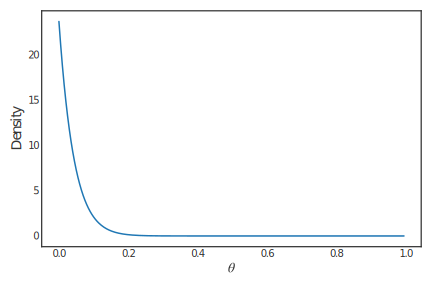
\includegraphics{images/betaposterior.svg}
\caption{Plot of the $\mathrm{Beta}(1,24)$ posterior density function}
\label{fig:ci1}

\end{figure}
Determine the $100(1-\alpha)\%$ HDI for~$\theta$.



!!dropdown!!

The HDI must include those values of $\theta$ with highest
    posterior density and so must take the form $C_\alpha=(0,b)$. The
    end-point $b$ must satisfy
    \begin{equation*}
    \int_0^b 24\,(1-\theta)^{23}\,d\theta = 1-\alpha.
    \end{equation*}
    Now
    \begin{equation*}
    \int_0^b 24\,(1-\theta)^{23}\,d\theta 
    = \left[-(1-\theta)^{24}\right]^b_0 = 1-(1-b)^{24}.
    \end{equation*}
    Hence
    $$
    1-(1-b)^{24}=1-\alpha \quad\Longrightarrow \quad 1-b=\alpha^{1/24}
    \quad\Longrightarrow \quad b=1-\alpha^{1/24}.
    $$
    Therefore, a $100(1-\alpha)\%$ HDI for $\theta$ is
    $(0,1-\alpha^{1/24})$.

!!enddropdown!!}



\paragraph{Example 4.2}{~\\
Suppose we have a random sample $\underline{x} = (x_1, \ldots, x_n)^\top$ from a $\mathcal{N}(\mu,1/\tau)$
distribution (where $\tau$ is known). We have seen that, assuming
vague prior knowledge, the posterior distribution is $\mu|\underline{x}\sim
\mathcal{N}(\bar x,1/(n\tau))$. Determine the $100(1-\alpha)\%$ HDI for~$\mu$.

!!dropdown!!

This distribution has a symmetric bell shape and so the HDI takes the
    form $C_\alpha=(a,b)$ with end-points
    $$
    a=\bar x - \frac{z_{\alpha/2}}{\sqrt{n\tau}}
    \quad\quad\text{and}\quad\quad
    b=\bar x + \frac{z_{\alpha/2}}{\sqrt{n\tau}},
    $$
    where $z_\alpha$ is the upper $\alpha$-quantile of the $\mathcal{N}(0,1)$
    distribution. Therefore, the 95\% HDI for~$\mu$ is 
    $$
    \left(\bar x - \frac{1.96}{\sqrt{n\tau}},\,
    \bar x + \frac{1.96}{\sqrt{n\tau}}\right).
    $$ 
    Note that this interval is numerically identical to the 95\% frequentist confidence interval for the (population) mean of a normal random sample with known variance. However, the interpretation is very
    different.

!!enddropdown!!}



\paragraph{Example 4.3}{~\\
Suppose that the posterior distribution for $\theta$ is a
\label{ex:hdi}
$\mathrm{Beta}(2,23)$ distribution, with probability density function
$$
\pi(\theta|\underline{x})=552\,\theta(1-\theta)^{22}, \quad 0<\theta<1.
$$
A plot of this distribution is given in Figure \ref{fig:ci2}.
\begin{figure}[h!]

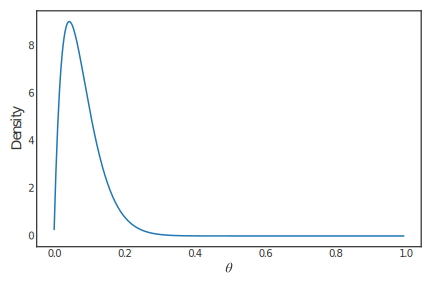
\includegraphics{images/betaposterior2.svg}
\caption{Plot of the $\mathrm{Beta}(2,23)$ posterior density function}
\label{fig:ci2}

\end{figure}
Determine the $100(1-\alpha)\%$ HDI for~$\theta$.

!!dropdown!!

Since the posterior density is unimodal, we seek $ 0 < a < b < 1 $ such that
    $$ \mathrm{Pr}(\theta \in (a,b)|\underline{x}) = 1 - \alpha $$
    and $\pi(a|\underline{x}) = \pi(b|\underline{x})$.
    
    Letting $F(a|\underline{x}) = \mathrm{Pr}(\theta < a|\underline{x})$ denote the posterior CDF, this is equivalent to  seeking $0<a<b<1$ such that
    $$ F(b|\underline{x}) - F(a|\underline{x}) = 1 - \alpha$$
    and $\pi(a|\underline{x}) = \pi(b|\underline{x})$.

!!enddropdown!!
\clearpage

\subsection*{Computation of HDIs for unimodal distributions}
Suppose that we require the HDI ($a,b$) for a unimodal distribution
with density $f(\cdot)$ and distribution function $F(\cdot)$.  We have
seen that if one of the end-points is known (because of the shape of
the distribution) or the distribution is symmetric then the solution
is in terms of the distribution's percentage points. When this is not
the case, the problem requires a numerical scheme to find $a$ and
$b$ satisfying
$$
F(b)-F(a)=1-\alpha \quad\quad\text{and}\quad\quad f(a)=f(b).
$$
The solution can be found by noticing that it also minimizes the
function
$$
g(a,b)=\bigl\{F(b)-F(a)-(1-\alpha)\bigr\}^2+k\bigl\{f(b)-f(a)\bigr\}^2,
$$
where $k>0$ is a tuning parameter that tries to ensure that both terms
are zeroed.  Therefore, we can used the \texttt{R} optimizer function
\texttt{optim} to determine $a$ and $b$.

\subsection*{Example~\ref{ex:hdi} (continued)}
Suppose we need the 95\% HDI for $\theta$ when $\theta|\underline{x}\sim \mathrm{Beta}(2,23)$. One slight complication with using the above method to determine the HDI $(a,b)$ is that both $a$ and $b$ are restricted to the unit interval. However, the \texttt{R} function \texttt{optim} has options for dealing with such cases. It also needs initial guesses at the values of $a$ and $b$. Here we base these on the values of the 95\% equi-tailed Bayesian credible interval. We also take $k=0.0001$ to balance the conditions to be zeroed.

The \texttt{R} code to determine $a$ and $b$ is 
\begin{minted}{Python}
g = function(x){
    a=x[1]
    b=x[2]
    g1 = (pbeta(b,2,23) - pbeta(a,2,23) - 0.95)^2
    g2 = 0.0001 * (dbeta(b,2,23) - dbeta(a,2,23))^2
    return(g1 + g2)
}

initiala=qbeta(0.025,2,23)
initialb=qbeta(0.975,2,23)
res=optim(c(initiala,initialb),g,method="L-BFGS-B",lower=0,upper=1)
a=res$par[1] 
b=res$par[2]
\end{minted}
and gives $a=0.002211733$ and $b=0.1840109$, with $F(b)-F(a)=0.9500041$ and $f(b)-f(a)=-0.004484121$. Thus the 95\% HDI is $(0.002211733,0.1840109)$.}



\section{Section 4.2: Prediction}
Much of statistical inference (both Frequentist and Bayesian) is aimed towards making statements about a parameter $\theta$. Often the inferences are used as a yardstick for similar future experiments. For example, we may want to predict the outcome when the experiment is performed again.

Clearly there will be uncertainty about the future outcome of an experiment. Suppose this future outcome $Y$ is described by a probability (density) function $f(y|\theta)$. There are several ways we could make inferences about what values of $Y$ are likely. For example, if we have an estimate $\hat{\theta}$ of $\theta$ we might base our inferences on $f(y|\theta=\hat{\theta})$. Obviously this is not the best we can do, as such inferences ignore the fact that it is very unlikely that $\theta=\hat{\theta}$. 

Implicit in the Bayesian framework is the concept of the {\it predictive distribution}. This distribution describes how likely are different outcomes of a future experiment. The predictive probability (density) function is calculated as
\begin{equation*}
f(y|\underline{x})=\int_\Theta
f(y|\theta)\,\pi(\theta|\underline{x})\,d\theta
\end{equation*}
when $\theta$ is a continuous quantity. From this equation, we can see that the predictive distribution is formed by weighting the possible values of $\theta$ in the future experiment $f(y|\theta)$ by how likely we believe they are to occur $\pi(\theta|\underline{x})$.

If the true value of $\theta$ were known, say $\theta_0$, then any prediction can do no better than one based on $f(y|\theta=\theta_0)$. However, as (generally) $\theta$ is unknown, the predictive distribution is used as the next best alternative.

We can use the predictive distribution to provide a useful range of plausible values for the outcome of a future experiment. This \emph{prediction interval} is similar to a HDI interval. A $100(1-\alpha)\%$ \emph{prediction interval} for $Y$ is the region $C_\alpha=\{y:~f(y|\underline{x})\geq\gamma\}$ where $\gamma$ is chosen so that $\text{Pr}(Y\in C_\alpha|\underline{x})=1-\alpha$.

\paragraph{Example 4.4}{~\\
Suppose that $X$ is the number of expensive goods sold in a shop over 24 days. If $\theta$ is the expected number of sales per day then it may be plausible that $X|\theta\sim Po(24\,\theta)$. Also, suppose our prior distribution for $\theta$ is as given in Table~\ref{tab:predprior}.

\begin{table}[ht]
\bigskip

\begin{tabular}{|c|c|c|}
\cline{2-3}
\multicolumn{1}{c|}{~}& $\theta$ & $\pi(\theta)$ \\
\hline
``great'' & 1/2 & 0.2 \\
``good'' & 1/4 & 0.5 \\
``poor'' & 1/8 & 0.3 \\
\hline
\end{tabular}
\caption{Prior distribution for $\theta$}
\label{tab:predprior}

\end{table}

Clearly, we believe that the most likely value of $\theta$ is 1/4, indicating that we would expect around 6 expensive goods to be sold in any 24 day period. Suppose now that we observe that $x=10$ expensive goods were sold in the last 24 days. This will impact our beliefs about $\theta$. We can calculate the posterior distribution for
$\theta$ as follows. The likelihood term is
\begin{align*}
\text{Pr}(X=10|\theta)
=\frac{(24\theta)^{10} e^{-24\theta}}{10!} 
&=\begin{cases} 0.1048 & \text{if }\theta=1/2 \\
                 0.0413 & \text{if }\theta=1/4 \\
                 0.0008 & \text{if }\theta=1/8\\
   \end{cases}
\end{align*}
and so, using Bayes Theorem
\begin{align*}
\pi(\theta=1/2|x=10)&=\frac{\text{Pr}(X=10|\theta=1/2)\pi(\theta=1/2)}
{[\text{Pr}(X=10|\theta=1/2)\pi(\theta=1/2)+\text{Pr}(X=10|\theta=1/4)\pi(\theta=1/4)} +\text{Pr}(X=10|\theta=1/8)\pi(\theta=1/8)] \\
& \\
&=\frac{0.1048\times 0.2}{0.1048\times 0.2+0.0413\times
0.5+0.0008\times 0.3} \\ \\
&=0.501 \\ \\
\pi(\theta=1/4|x=10)&=\cdots=0.493 \\
\pi(\theta=1/8|x=10)&=\cdots=0.006.
\end{align*}
Thus, the posterior distribution for $\theta$ is as shown in Table \ref{tab:predpost}, with most likely value of $\theta$ now being 1/2, and standard deviation $\textnormal{SD}(\theta|x=10)=0.126$.
\begin{table}[ht]
\bigskip

\begin{tabular}{|c|c|c|}
\cline{2-3}
\multicolumn{1}{c|}{~}& $\theta$ & $\pi(\theta|x=10)$ \\
\hline
``great'' & 1/2 & 0.501 \\
``good''  & 1/4 & 0.493 \\
``poor''  & 1/8 & 0.006 \\
\hline
\end{tabular}
\caption{Posterior distribution for $\theta$}
\label{tab:predpost}

\end{table}

Suppose now we want to predict the number of sales $Y$ in the next 24
days. If there have been no changes in the sales process (no special
advertising campaigns etc) then we can take $Y|\theta\sim
\mathrm{Poisson}(24\,\theta)$. Determine the predictive probability function for~$Y$.



\clearpage

!!dropdown!!

As $\theta$ is discrete, the predictive probability
        function for $Y$ is
        \begin{align*}
        f(y&|x=10)\\
        &=\sum_{\theta=\frac{1}{2},\frac{1}{4},\frac{1}{8}} 
        f(y|\theta)\,\pi(\theta|x=10) \\
        &=\left(0.501\times\frac{12^ye^{-12}}{y!}\right) +
        \left(0.493\times\frac{6^ye^{-6}}{y!}\right)+
        \left(0.006\times\frac{3^ye^{-3}}{y!}\right) \\
        &=\frac{0.501\times 12^ye^{-12}+0.493\times 6^ye^{-6}+0.006\times 3^ye^{-3}}
        {y!}
        \end{align*}
        For example
        \begin{align*}
        \text{Pr}(Y=10|x=10)&=
        \frac{0.501\times 12^{10}e^{-12}+0.493\times 6^{10}e^{-6}+
        0.006\times 3^{10}e^{-3}}{10!}\\
        &=0.073.
        \end{align*}

!!enddropdown!!

This probability can be compared with a more naive predictive
probability calculated assuming that $\theta=\hat{\theta}$, the
likelihood mode. Here $\hat{\theta}=1/2$ and so $Y|\theta=\hat{\theta}\sim
Po(24\hat{\theta})\equiv Po(12)$, whence
\begin{equation*}
\text{Pr}(Y=10|\theta=\hat{\theta})=\frac{12^{10} e^{-12}}{10!}=0.1048.
\end{equation*}

In the same manner, we can calculate the entire predictive distribution
and naive predictive distribution; see Table~\ref{tab:predsimple}.



\begin{table}[ht]
\bigskip

\begin{tabular}{|r|c|c|}
\cline{2-3}
\multicolumn{1}{c|}{~}& correct & naive \\
\cline{1-1}
$y$ & $f(y|x=10)$ & $f(y|\theta=\hat{\theta})$ \\
\hline
0 & 0.002 & 0.000 \\
1 & 0.008 & 0.000 \\
2 & 0.024 & 0.000 \\
3 & 0.046 & 0.002 \\
4 & 0.070 & 0.005 \\
5 & 0.086 & 0.013 \\
6 & 0.092 & 0.025 \\
7 & 0.090 & 0.044 \\
8 & 0.084 & 0.066 \\
9 & 0.078 & 0.087 \\
10 & 0.073 & 0.105 \\
11 & 0.068 & 0.114 \\
12 & 0.063 & 0.114 \\
13 & 0.055 & 0.106 \\
14 & 0.046 & 0.090 \\
15 & 0.037 & 0.072 \\
16 & 0.027 & 0.054 \\
17 & 0.019 & 0.038 \\
18 & 0.013 & 0.026 \\
19 & 0.008 & 0.016 \\
20 & 0.005 & 0.010 \\
$\vdots$ & $\vdots$ & $\vdots$ \\
\hline
\end{tabular}
\caption{Predictive and ``naive'' predictive probability functions}
\label{tab:predsimple}

\end{table}
Notice that the correct predictive probability distribution has more
probability out in the tails of its distribution, that is, the
probabilities of 0, 1, 2, $\ldots$ are larger than their ``naive''
equivalents. This is a common occurrence. It is due to ignoring the
uncertainty about the parameter estimate. Essentially, the naive
predictive distribution is a predictive distribution which, instead of
using the correct posterior distribution, uses the degenerate
posterior distribution
\begin{equation*}
\pi^*(\theta|x=10)=\begin{cases} 1 & \text{if } \theta=1/2 \\
                                 0 & \text{otherwise}, \\
              \end{cases}
\end{equation*}
a distribution with standard deviation $\textnormal{SD}_{\pi^*}(\theta|x=10)=0$.
The correct posterior standard deviation of $\theta$ is
$\textnormal{SD}_\pi(\theta|x=10)=0.126$.  Therefore, the predictive distribution
using the naive posterior $\pi^*$ is, loosely speaking, too confident
that it ``knows'' the value of $\theta$ and so produces a predictive
distribution with too small a standard deviation:
\begin{equation*}
\textnormal{SD}(Y|x=10)=
\begin{cases} 4.26  & \text{using the correct }\pi(\theta|x=10) \\
              3.46  & \text{using the naive }\pi^*(\theta|x=10). \\
         \end{cases}
\end{equation*}
These standard deviations can be calculated from
Table~\ref{tab:predsimple}. 



We can also use the above table of predictive probabilities to determine a
prediction interval for $Y$. Using the correct predictive
distribution, and recalling the highest density feature of prediction
intervals, we obtain $\text{Pr}(2\leq Y\leq 17|x=10)=0.959$. The
corresponding naive calculation is $\text{Pr}(6\leq Y\leq
19|\theta=\hat{\theta})=0.958$. Hence the correct (approximate) 96\%
prediction interval for $Y$ is $\{2,3,\ldots,17\}$. The naive version,
and hence narrower interval, is $\{6,7,\ldots,19\}$.}

\paragraph{Definition 4.1: Definition}{~\\
The random variable $Y$ follows a Beta-binomial $\mathrm{BetaBin}(n,a,b)$
distribution ($n$ positive integer, $a>0$, $b>0$) if it has
probability function
$$f(y|n,a,b)=\binom{n}{y}\frac{\mathrm{B}(y+a,b+n-y)}{\mathrm{B}(a,b)}, \quad\quad
y=0,1,\ldots,n,$$ 
where $\mathrm{B}(a,b)$ is the beta function defined in \eqref{eq:betafn}. It can be shown that
$$\text{E}[Y] =\frac{na}{a+b}\quad\quad\text{and}\quad\quad
\text{Var}[Y]=\frac{nab(a+b+n)}{(a+b)^2(a+b+1)}. $$}

\paragraph{Example 4.5}{~\\
Suppose that $X$ is the number of defective items in a sample of
size~5. If the items are defective independently of one another and
they each have the same probability $\theta$ of being defective then
$X|\theta\sim \mathrm{Bin}(5,\theta)$. Suppose we believe that defective items
are quite unlikely and so take a $\mathrm{Beta}(1,19)$ prior distribution with
mean and standard deviation
\begin{equation*}
\text{E}[\theta]=0.05\quad\quad\text{and}\quad\quad \textnormal{SD}(\theta)=0.048.
\end{equation*}
Suppose we take a sample of size~5 and observe $x=1$ defective item.
In this case, the likelihood mode is $\hat{\theta}=1/5=0.2$, higher than
the prior mean. We have seen previously that, in such cases, the
posterior distribution is a $\mathrm{Beta}$ distribution whose first and second
parameters are those of the prior distribution incremented by the
number of success and the number of failures respectively. Thus, the
posterior distribution is a $\mathrm{Beta}(2,23)$ distribution, with mean and
standard deviation
$$
\text{E}[\theta|x=1]=0.08\quad\quad\text{and}\quad\quad \textnormal{SD}(\theta|x=1)=0.053.
$$
The posterior mean is larger than the prior mean and the standard
deviation has also increased (slightly).

If we observe another sample of 5 items, what is the predictive
probability distribution of the number found to be defective?

\clearpage

!!dropdown!!

Suppose the number of defective items in this future sample is $Y$, with $Y|\theta\sim \mathrm{Bin}(5,\theta)$. The predictive probability function of $Y$ is, for $y=0,1,2,\ldots,5$
    \begin{align*}
    f(y|x=1)
    &=\int_\Theta f(y|\theta)\,\pi(\theta|x=1)\,d\theta \\
    &=\int_0^1 \binom{5}{y}\theta^y(1-\theta)^{5-y}
    \times \frac{\theta(1-\theta)^{22}}{\mathrm{B}(2,23)}\,d\theta \\
    &=\binom{5}{y}\frac{1}{\mathrm{B}(2,23)}
    \int_0^1 \theta^{y+1}(1-\theta)^{27-y}\,d\theta \\
    &=\binom{5}{y}\frac{\mathrm{B}(y+2,28-y)}{\mathrm{B}(2,23)},
    \end{align*}
    That is, $Y|x=1\sim \mathrm{BetaBin}(5,2,23)$.

!!enddropdown!!}

We can compare this predictive distribution with a naive predictive distribution based on an estimate of $\theta$, for example, the likelihood mode or the posterior mode. Here we shall base our naive predictive distribution on the posterior mode $\hat{\theta}=1/23$, that is, use the distribution $Y|\theta=\hat\theta\sim \mathrm{Bin}(5,1/23)$. Thus, the naive predictive probability function is, for $y=0,1,\ldots,5$,
\begin{align*}
f(y|\theta=\hat{\theta})&=\binom{5}{y}\hat{\theta}^y(1-\hat{\theta})^{5-y} 
=\binom{5}{y}\frac{22^{5-y}}{23^5}.
\end{align*}

Numerical values for the predictive and naive predictive probability functions are given in Table~\ref{tab:predbetabin}.
\begin{table}[ht]
\bigskip

\begin{tabular}{|r|c|c|}
\cline{2-3}
\multicolumn{1}{c|}{~}& correct & naive \\
\cline{1-1}
$y$ & $f(y|x=1)$ & $f(y|\theta=\hat{\theta})$ \\
\hline
0 & 0.680 & 0.801 \\
1 & 0.252 & 0.182 \\
2 & 0.058 & 0.017 \\
3 & 0.009 & 0.001 \\
4 & 0.001 & 0.000 \\
5 & 0.000 & 0.000 \\
\hline
\end{tabular}

\caption{Predictive and naive predictive probability functions}
\label{tab:predbetabin}
\end{table}
Again, the naive predictive distribution is a predictive
distribution which, instead of using the correct posterior
distribution, uses a degenerate posterior distribution
$\pi^*(\theta|x=1)$ which essentially allows only one value: $\text{Pr}_{\pi^*}(\theta=1/23|x=1)=1$ and
standard deviation $\textnormal{SD}_{\pi^*}(\theta|x=1)=0$. Note that the correct
posterior standard deviation of $\theta$ is
$\textnormal{SD}_\pi(\theta|x=1)=0.053$. Using a degenerate posterior distribution
results in the naive predictive distribution having too small a
standard deviation:
\begin{equation*}
\textnormal{SD}(Y|x=1)=
\begin{cases} 0.652 & \text{using the correct }\pi(\theta|x=1) \\
              0.456 & \text{using the naive }\pi^*(\theta|x=1), \\
\end{cases}
\end{equation*}
these values being calculated from $\mathrm{BetaBin}(5,2,23)$ and binomial
$\mathrm{Bin}(5,1/23)$ distributions.

Using the numerical table of predictive probabilities, we can see that
$\{0,1\}$ is a 93.2\% prediction set/interval. This is to be
contrasted with the more ``optimistic'' calculation using the naive
predictive distribution which shows that $\{0,1\}$ is a 98.3\%
prediction set/interval.

\clearpage

\subsection*{Predictive distribution}
In the previous example, a non-trivial integral had to be evaluated.
However, when the past data $\underline{x}$ and future data $y$ are
independent (given $\theta$) and we use a conjugate prior
distribution, another (easier) method can be used to determine the
predictive distribution.

Using Bayes Theorem, the posterior density for $\theta$ given
$\underline{x}$ and $y$ is
\begin{align*}
\pi(\theta|\underline{x},y)&=\frac{\pi(\theta)f(\underline{x},y|\theta)}{f(\underline{x},y)}\\
&=\frac{\pi(\theta)f(\underline{x}|\theta)f(y|\theta)}{f(\underline{x})f(y|\underline{x})}
\\
&=\frac{\pi(\theta|\underline{x})\,f(y|\theta)}{f(y|\underline{x})}.
\end{align*}
Rearranging, we obtain:
$$f(y|\underline{x}) =\frac{f(y|\theta)\pi(\theta|\underline{x})}{\pi(\theta|\underline{x},y)}.$$
The right-hand-side of this equation looks as if it depends on
$\theta$, but, in fact, any terms in $\theta$ will be cancelled
between the numerator and denominator.

Reworking the previous example using this formula, we have
$$
\theta\sim \mathrm{Beta}(1,19),\quad X|\theta\sim \mathrm{Bin}(5,\theta),\quad 
Y|\theta\sim \mathrm{Bin}(5,\theta)
$$
from which we obtain
$$
\theta|x=1\sim \mathrm{Beta}(2,23),\quad \theta|x=1,y\sim \mathrm{Beta}(y+2,28-y).
$$
Therefore, for $y=0,1,2,\ldots,5$
\begin{align*}
f(y|x=1)&=\frac{f(y|\theta)\pi(\theta|x=1)}{\pi(\theta|x=1,y)}\\
{}
&=\frac{\begin{pmatrix} 5 \\ y \\ \end{pmatrix} 
\theta^y(1-\theta)^{5-y}
\times \frac{\theta(1-\theta)^{22}}{\mathrm{B}(2,23)}}
{\frac{\theta^{y+1}(1-\theta)^{27-y}}{\mathrm{B}(y+2,28-y)}}\\ 
{}
&=\begin{pmatrix} 5 \\ y \\ \end{pmatrix} \frac{\mathrm{B}(y+2,28-y)}{\mathrm{B}(2,23)}.
\end{align*}

\clearpage

\paragraph{Definition 4.2: Inverse-Beta Distribution}{~\\
The random variable $Y$ follows a Inverse-Beta distribution, denoted $Y\sim\mathrm{InvBeta}(a,b,c)$ with parameters $a>0$, $b>0$ and $c>0$,  if it has probability density function
$$
f(y|a,b,c)=\frac{c^by^{a-1}}{\mathrm{B}(a,b)(y+c)^{a+b}} \quad\quad y>0, 
$$
where $\mathrm{B}(a,b)$ is the beta function defined in
\eqref{eq:betafn}. It can be shown that
$$\text{E}[Y]=\frac{ac}{b-1}\quad\quad\text{and}\quad\quad \text{Var}[Y]=\frac{ac^2(a+b-1)}{(b-1)^2(b-2)}.$$
The distribution gets its name because $Y/(Y+c)\sim \mathrm{Beta}(a,b)$. Also note that if $Y\sim \mathrm{InvBeta}(a,b,1)$ then $cY\sim \mathrm{InvBeta}(a,b,c)$.}

\clearpage

\paragraph{Example 4.6}{~\\
  Suppose we have a random sample $\underline{x} = (x_1, \ldots, x_n)^\top$ from a $\mathrm{Gamma}(k,\theta)$
  distribution, where $k$ is known, and our prior beliefs are
  described by a $\mathrm{Gamma}(g,h)$ distribution. The likelihood function is
$$ f(\underline{x}|\theta)=\prod_{i=1}^n \frac{\theta^k x_i^{k-1}e^{-\theta x_i}}{\Gamma(k)}\propto\theta^{nk}e^{-n\bar x\theta}.$$
 Therefore, using Bayes Theorem, the posterior density is
 \begin{align*}
  \pi(\theta|\underline{x}) &\propto\pi(\theta)\,f(\underline{x}|\theta) \\
  &\propto\theta^{g-1}e^{-h\theta}\times\theta^{nk}e^{-n\bar x\theta}, \quad\theta>0 \\
  &\propto\theta^{g+nk-1}e^{-(h+n\bar x)\theta},\quad\theta>0.
\end{align*}
Hence, the posterior distribution is a $\mathrm{Gamma}(g+nk,h+n\bar x)$ distribution. Notice that this implies that the gamma distribution is the conjugate prior distribution for the model ``random sample from a $\mathrm{Gamma}(k,\theta)$ distribution, with $k$ known''. Determine the predictive distribution for a future outcome~$Y$.



\clearpage

!!dropdown!!

Clearly, the posterior distribution for $\theta$ conditional on both
    the data $\underline{x}$ and the future observation~$y$ is given by
    $\theta|\underline{x},y\sim \mathrm{Gamma}(G+k,H+y)$. Therefore, the predictive density
    function is, for $y>0$
    \begin{align*}
    f(y|\underline{x})&=\frac{f(y|\theta)\pi(\theta|\underline{x})}{\pi(\theta|\underline{x},y)}\\
    {}
    &=\frac{\frac{\theta^k y^{k-1}e^{-\theta y}}{\Gamma(k)}
    \times \frac{H^G\theta^{G-1}e^{-H\theta}}{\Gamma(G)}}
    {\frac{(H+y)^{G+k}\theta^{G+k-1}e^{-(H+y)\theta}}{\Gamma(G+k)}}\\
    {}
    &=\frac{\Gamma(G+k)H^Gy^{k-1}}{\Gamma(k)\Gamma(G)(H+y)^{G+k}}\\ 
    {}
    &=\frac{H^Gy^{k-1}}{\mathrm{B}(k,G)(H+y)^{G+k}},
    \end{align*}
    That is, $Y|\underline{x}\sim \mathrm{InvBeta}(k,G,H)$. \\ 
    Consider the case where the data follow an exponential distribution, that is, where $k=1$. Determine the predictive density function and the $100(1-\alpha)\%$ prediction interval for~$Y$.

!!enddropdown!!}

\clearpage

\thispagestyle{empty}
\vspace*{0.25\textheight}

\bfseries\fontsize{60pt}{60pt}\selectfont The End
